\documentclass{article}
\usepackage[paperwidth=13.2in,paperheight=6.85in,margin=0.10in]{geometry}
\usepackage{amsmath}
\usepackage{tikz}
\usetikzlibrary{arrows.meta,positioning,calc}
\pagestyle{empty}

\begin{document}
\noindent
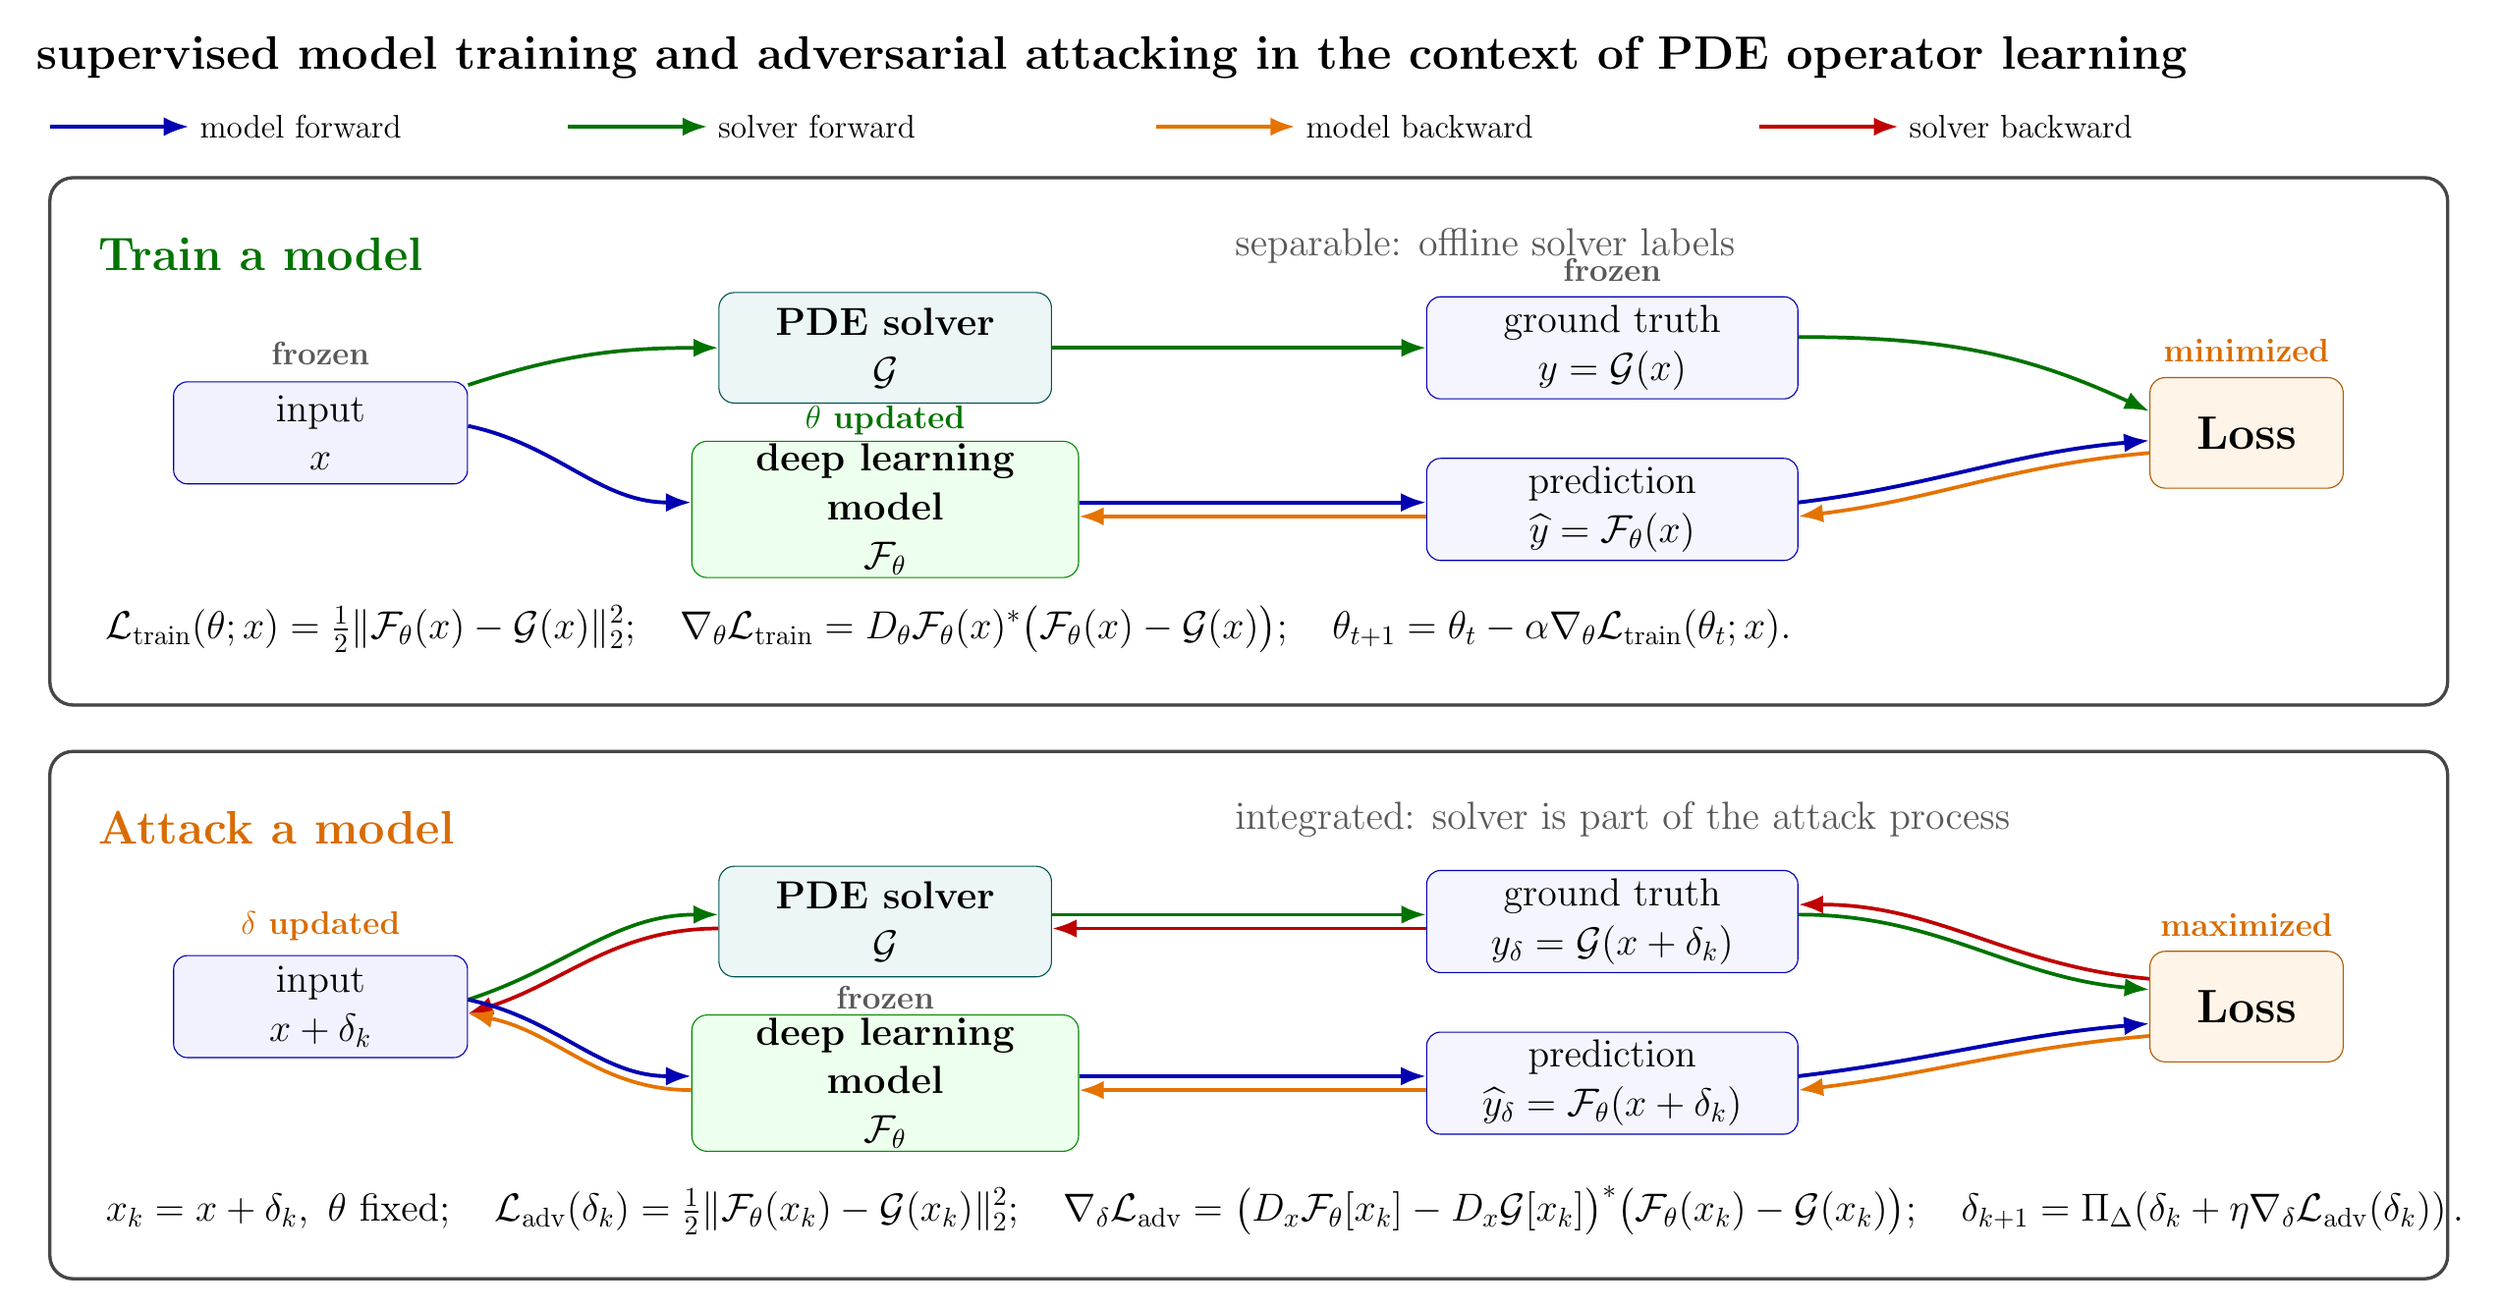
\begin{tikzpicture}[
  x=1mm,y=1mm,
  >=Latex,
  font=\sffamily,
  panel/.style={draw=black!55, rounded corners=3mm, line width=0.9pt, fill=white},
  input/.style={draw=blue!70!black, rounded corners=1.8mm, fill=blue!5, minimum width=38mm, minimum height=13.2mm, align=center, font=\Large, inner ysep=1pt},
  solver/.style={draw=teal!65!black, rounded corners=2mm, fill=teal!7, minimum width=43mm, minimum height=14.3mm, align=center, font=\Large\bfseries, inner ysep=1pt},
  model/.style={draw=green!55!black, rounded corners=2mm, fill=green!7, minimum width=50mm, minimum height=16.5mm, align=center, font=\Large\bfseries, inner ysep=1pt},
  outbox/.style={draw=blue!70!black, rounded corners=1.8mm, fill=blue!4, minimum width=48mm, minimum height=13.2mm, align=center, font=\Large, inner ysep=1pt},
  loss/.style={draw=orange!70!black, rounded corners=2mm, fill=orange!9, minimum width=25mm, minimum height=14.3mm, align=center, font=\LARGE\bfseries, inner ysep=1pt},
  label/.style={font=\LARGE\bfseries, anchor=west},
  formula/.style={font=\Large, anchor=south west, align=left},
  note/.style={font=\large, text=black!65, align=left},
  smallnote/.style={font=\large\bfseries, text=black!65, align=center, anchor=south},
  captionnote/.style={font=\Large, text=black!65, align=center},
  action/.style={font=\large\bfseries, align=center, anchor=south},
  fwd/.style={->, draw=blue!70!black, line width=1.4pt},
  bmodel/.style={->, draw=orange!90!black, line width=1.35pt},
  solverline/.style={->, draw=green!45!black, line width=1.35pt},
  bsolver/.style={->, draw=red!75!black, line width=1.35pt}
]

% Title and legend
\node[font=\LARGE\bfseries, anchor=west] at (5,168)
  {supervised model training and adversarial attacking in the context of PDE operator learning};
\draw[fwd] (8,159) -- ++(18,0) node[right, black, font=\large] {model forward};
\draw[solverline] (75,159) -- ++(18,0) node[right, black, font=\large] {solver forward};
\draw[bmodel] (151,159) -- ++(18,0) node[right, black, font=\large] {model backward};
\draw[bsolver] (229,159) -- ++(18,0) node[right, black, font=\large] {solver backward};

% ================= Panel 1 =================
\begin{scope}[shift={(0,84.2)}]
  \draw[panel] (8,0) rectangle (318,68.2);
  \node[label, text=green!45!black] at (13,58.3) {Train a model};
  \node[captionnote, anchor=west, text=black!65] at (160,59.4)
    {separable: offline solver labels};
  \node[formula] at (14,5.5)
    {$\displaystyle
      \mathcal L_{\mathrm{train}}(\theta;x)=\tfrac12\|\mathcal F_\theta(x)-\mathcal G(x)\|_2^2;\quad
      \nabla_\theta\mathcal L_{\mathrm{train}}
      =D_\theta\mathcal F_\theta(x)^*\bigl(\mathcal F_\theta(x)-\mathcal G(x)\bigr);\quad
      \theta_{t+1}=\theta_t-\alpha\nabla_\theta\mathcal L_{\mathrm{train}}(\theta_t;x).$};

  \node[input] (xin) at (43,35.2) {input\\$x$};
  \node[solver] (solver) at (116,46.2) {PDE solver\\$\mathcal G$};
  \node[model] (model) at (116,25.3) {deep learning\\model\\$\mathcal F_\theta$};
  \node[outbox] (ygt) at (210,46.2) {ground truth\\$y=\mathcal G(x)$};
  \node[outbox] (ypred) at (210,25.3) {prediction\\$\widehat y=\mathcal F_\theta(x)$};
  \node[loss] (loss) at (292,35.2) {Loss};

  \node[smallnote] at (43,42.7) {frozen};
  \node[smallnote, text=green!45!black] at (116,33.7) {$\theta$ updated};
  \node[smallnote] at (210,53.5) {frozen};
  \node[action, text=orange!85!black] at (292,43.1) {minimized};

  \draw[solverline] (xin) to[out=18,in=180] (solver);
  \draw[solverline] (solver) -- (ygt);
  \draw[fwd] ([yshift=0.9mm]xin.east) to[out=-12,in=180] ([yshift=0.9mm]model.west);
  \draw[fwd] ([yshift=0.9mm]model.east) -- ([yshift=0.9mm]ypred.west);
  \draw[solverline] ([yshift=1.4mm]ygt.east)
    to[out=0,in=155] ([yshift=2.8mm]loss.west);
  \draw[fwd] ([yshift=0.9mm]ypred.east) to[out=7,in=185] ([yshift=-1.0mm]loss.west);

  \draw[bmodel] ([yshift=-2.6mm]loss.west)
    to[out=185,in=7] ([yshift=-0.9mm]ypred.east);
  \draw[bmodel] ([yshift=-0.9mm]ypred.west)
    -- ([yshift=-0.9mm]model.east);
\end{scope}

% ================= Panel 2 =================
\begin{scope}[shift={(0,10)}]
  \draw[panel] (8,0) rectangle (318,68.2);
  \node[label, text=orange!85!black] at (13,58.3) {Attack a model};
  \node[captionnote, anchor=west, text=black!65] at (160,59.4)
    {integrated: solver is part of the attack process};
  \node[formula] at (14,4.4)
    {$\displaystyle
      x_k=x+\delta_k,\ \theta\ \mathrm{fixed};\quad
      \mathcal L_{\mathrm{adv}}(\delta_k)=\tfrac12\|\mathcal F_\theta(x_k)-\mathcal G(x_k)\|_2^2;\quad
      \nabla_\delta\mathcal L_{\mathrm{adv}}
      =\bigl(D_x\mathcal F_\theta[x_k]-D_x\mathcal G[x_k]\bigr)^*
      \bigl(\mathcal F_\theta(x_k)-\mathcal G(x_k)\bigr);\quad
      \delta_{k+1}=\Pi_\Delta\!\left(\delta_k+\eta\nabla_\delta\mathcal L_{\mathrm{adv}}(\delta_k)\right).$};

  \node[input] (xin) at (43,35.2) {input\\$x+\delta_k$};
  \node[solver] (solver) at (116,46.2) {PDE solver\\$\mathcal G$};
  \node[model] (model) at (116,25.3) {deep learning\\model\\$\mathcal F_\theta$};
  \node[outbox] (ygt) at (210,46.2) {ground truth\\$y_\delta=\mathcal G(x+\delta_k)$};
  \node[outbox] (ypred) at (210,25.3) {prediction\\$\widehat y_\delta=\mathcal F_\theta(x+\delta_k)$};
  \node[loss] (loss) at (292,35.2) {Loss};

  \node[smallnote, text=orange!85!black] at (43,42.5) {$\delta$ updated};
  \node[smallnote] at (116,33.7) {frozen};
  \node[action, text=orange!85!black] at (292,43.1) {maximized};

  \draw[solverline] ([yshift=0.9mm]xin.east) to[out=18,in=180] ([yshift=0.9mm]solver.west);
  \draw[solverline] ([yshift=0.9mm]solver.east) -- ([yshift=0.9mm]ygt.west);
  \draw[solverline] ([yshift=0.9mm]ygt.east) to[out=0,in=175] ([yshift=2.2mm]loss.west);
  \draw[bsolver] ([yshift=3.6mm]loss.west) to[out=175,in=0] ([yshift=2.2mm]ygt.east);
  \draw[bsolver] ([yshift=-0.9mm]ygt.west) -- ([yshift=-0.9mm]solver.east);
  \draw[bsolver] ([yshift=-0.9mm]solver.west) to[out=180,in=18] ([yshift=-0.9mm]xin.east);
  \draw[fwd] ([yshift=0.9mm]xin.east) to[out=-12,in=180] ([yshift=0.9mm]model.west);
  \draw[fwd] ([yshift=0.9mm]model.east) -- ([yshift=0.9mm]ypred.west);
  \draw[fwd] ([yshift=0.9mm]ypred.east) to[out=7,in=185] ([yshift=-2.2mm]loss.west);

  \draw[bmodel] ([yshift=-3.8mm]loss.west)
    to[out=185,in=7] ([yshift=-0.9mm]ypred.east);
  \draw[bmodel] ([yshift=-0.9mm]ypred.west)
    -- ([yshift=-0.9mm]model.east);
  \draw[bmodel] ([yshift=-0.9mm]model.west)
    to[out=180,in=-12] ([yshift=-0.9mm]xin.east);
\end{scope}

% Redraw panel borders on the foreground so the left edges remain solid in PDF/PNG output.
\draw[draw=black!72, rounded corners=3mm, line width=1.2pt, line join=round]
  (8,84.2) rectangle (318,152.4);
\draw[draw=black!72, line width=1.2pt, line cap=round] (8,88.2) -- (8,148.4);
\draw[draw=black!72, rounded corners=3mm, line width=1.2pt, line join=round]
  (8,10) rectangle (318,78.2);
\draw[draw=black!72, line width=1.2pt, line cap=round] (8,14) -- (8,74.2);

\end{tikzpicture}
\end{document}
